\documentclass[ignorenonframetext, professionalfonts, hyperref={pdftex, unicode}]{beamer}

\usetheme{Copenhagen}
\usecolortheme{wolverine}

\usepackage[orientation=landscape, size=custom, width=16, height=9.75, scale=0.5]{beamerposter}	

%Packages to be included

\usepackage{textcomp}

\usepackage[russian]{babel}
\usepackage[utf8]{inputenc}
\usepackage[T1]{fontenc}

\usepackage{beamerthemesplit}

\usepackage{ulem}

\usepackage{verbatim}

\usepackage{ucs}
\usepackage{listings}
\lstloadlanguages{C, make, bash}

\lstset{escapechar=`,
	extendedchars=false,
	language=C, 
	tabsize=2, 
	columns=fullflexible, 
%	basicstyle=\scriptsize,
	keywordstyle=\color{blue}, 
	commentstyle=\itshape\color{brown},
%	identifierstyle=\ttfamily, 
	stringstyle=\mdseries\color{green}, 
	showstringspaces=false, 
	numbers=left, 
	numberstyle=\tiny, 
	breaklines=true, 
	inputencoding=utf8x,
	keepspaces=true,
	morekeywords={u\_short, u\_char, u\_long, in\_addr}
	}

\definecolor{darkgreen}{cmyk}{0.7, 0, 1, 0.5}

\lstdefinelanguage{diff}
{
    morekeywords={+, -},
    sensitive=false,
    morecomment=[l]{//},
    morecomment=[s]{/*}{*/},
    morecomment=[l][\color{darkgreen}]{+},
    morecomment=[l][\color{red}]{-},
    morestring=[b]",
}



%%%%%%%%%%%%%%%%%%%%%%%%%%%%%%%%%%%%%%%%%%%%%%%%%
%%%%%%%%%% PDF meta data inserted here %%%%%%%%%%
%%%%%%%%%%%%%%%%%%%%%%%%%%%%%%%%%%%%%%%%%%%%%%%%%
\hypersetup{
	pdftitle={Введение в GNU/Linux},
	pdfauthor={Epam/LLPD}
}





%%%%%% Beamer Theme %%%%%%%%%%%%%

	
\title{Введение в GNU/Linux}
\author{Epam/LLPD}



%%%%%%%%%%%%%%%%%%%%%%%%%%%%%%%%%%%%%%%%%%%%%%%%%
%%%%%%%%%% Begin Document  %%%%%%%%%%%%%%%%%%%%%%
%%%%%%%%%%%%%%%%%%%%%%%%%%%%%%%%%%%%%%%%%%%%%%%%%




\begin{document}

%\section{Командная строка}


\frame{
	\frametitle{}
	\titlepage
	\vspace{-0.5cm}
	\begin{center}
	%\frontpagelogo
	\end{center}
}
\frame{
	\tableofcontents
%	[hideallsubsections]
}

%\subsection{Командная оболочка}
\begin{frame}[fragile]{Определение(не совсем формальное)}
\textbf{Shell} -- приложение, обеспечивающее выполнение других приложений и их взаимодействие, а также представляющая услуги командной строки. 
\begin{center}
  или
\end{center}
\textbf{Shell} -- приложение, обеспечивающее доступ к основным функциям ядра.

\pause
\vspace{0.5in}
Пример shell из Windows-world -- cmd.exe
\vspace{0.5in}

Минимальный дистрибутив Linux -- ядро + shell 

\end{frame}
\begin{frame}[fragile]{Основные типы shell в Unix}
  \begin{itemize}
    \item Bourne shell совместимые
      \begin{itemize}
        \item \textbf{sh} исходная bourne shell (Steve Bourne, 1978)
        \item \textbf{ksh} Korn shell (David Korn, 1983)
        \item \textbf{ash} $[$BSD$]$ Almquist shell (Kenneth Almquist,1989)  
        \item \textbf{bash} $[$GPL$]$ Bourne-again shell (Brian Fox, 1989)
        \item \textbf{zsh} $[$BSD$]$ Z shell (Paul Falstad,1990)
        \item \textbf{/bin/sh} Указывает на POSIX-совместимую shell
      \end{itemize}
  \item C shell совместимые
      \begin{itemize}
        \item \textbf{csh}  Исходная С shell (Bill Joy, 1978)
        \item \textbf{tcsh} $[$BSD$]$ TENEX C shell (Ken Greer, 1981)
       \end{itemize}
  \end{itemize}
\end{frame}
\begin{frame}[fragile]{Маленькое упражнение}
\begin{lstlisting}[language=bash]
cat /etc/shells
ls -l <filename> # для каждого элемента /etc/shells
readlink -e <filename> 
\end{lstlisting}
\end{frame}
%\subsection{bash -- Работа в командной строке}
\begin{frame}[fragile]{Получение помощи}
  \begin{itemize}
    \pause
    \item \textbf{man} - помощь по внешним командам
    \pause
    \item \textbf{help} - помощь по внутренним командам bash (также man bash)
    \pause
    \item \textbf{info} - расширенная помощь по некоторым командам (texinfo format)
      \begin{itemize}
       \item   Попробовать {\tt info coreutils}
       \item   Справка по навигации -- нажать h
      \end{itemize}
  \end{itemize}
\end{frame}
\begin{frame}[fragile]{Основное о man}
\begin{columns}
  \column{2.2in}
  \begin{itemize}
        \item Прочитайте {\tt man man} !
        \item Apropos {\tt man -k <слово>}
        \item Разделы (sections)
          \begin{itemize}
            \item[1] Основная секция(юзерские программы) 
            \item[2] Syscalls
            \item[3] С library
            \item[5] Конфигурационные файлы
            \item[8] Системные службы
          \end{itemize}
  \end{itemize}
  \textbf{Замечание}

  Обычно внутри страницы работает поиск с помощью '/'
 \pause 
 \column{1in}
 \begin{block}{Попробовать}
\begin{lstlisting}
man -k printf
man 3 printf
man 1 printf
man -a printf
\end{lstlisting}
\end{block}
\end{columns}
\end{frame}
\begin{frame}{Навигация по файловой системе}
      \begin{itemize}
        \item Список файлов в (текущей по умолчанию) директории  \textbf{ls} (man ls)
        \item Смена текущей директории \textbf{cd} (help cd)
        \item Имя текущей директории  \textbf{pwd} (help pwd)
      \end{itemize}
\end{frame}

\begin{frame}[fragile]{Команды для работы с файлами}
	\begin{itemize}
		\begin{columns}
		\column{0.2\textwidth}
			\item touch
			\item ln
			\item mkdir
			\item mknod
			\item mkfifo
		\column{0.2\textwidth}
			\item cp
			\item mv
			\item install
			\item rm
			\item rmdir
			\item file
		\column{0.4\textwidth}
			\begin{block}{Упражнение}
				Создать иерархию директорий

\begin{lstlisting}
dir1/dir1.1/dir1.1.1
dir1/dir1.2/dir1.2.1
dir1/dir1.2/dir1.2.2
\end{lstlisting}

				Внутри каждой создать файл

				Удалить все созданное
			\end{block}
		\end{columns}
	\end{itemize}
\end{frame}

\begin{frame}{Важные аббревиатуры внутри командной строки}
  \begin{itemize}
    \item Для директорий
      \begin{itemize}
        \item {\tt $\sim$} Домашняя директория
        \item {\tt $\sim$<username>} Домашняя директория пользователя
        \item {\tt ..} Родительская директория
        \item {\tt .} Текущая директория
      \end{itemize}
      \pause  
    \item Wildcards
      \begin{itemize}
        \item {\tt *} Любой набор символов {\tt file*txt : file1.txt filefilefiletxt}
        \item {\tt $[$<список>$]$ } символ из заданного набора {\tt }
        \item {\tt ?} любой один символ
      \end{itemize}

  \end{itemize}
\end{frame}       

\begin{frame}{Горячие клавиши}
  \begin{itemize}
    \item \textbf{Tab} -- дополнение текущей команды
      \pause
    \item История команд
      \begin{itemize}
        \item Клавиши курсора -- навигация по истории
        \item Ctrl-R -- поиск в истории по фрагменту
        \item Ctrl-O (после выполнения вставить следующую команду из истории)
        \item Команда {\tt history}
      \end{itemize}
    \item Навигация

  \end{itemize}
\end{frame}

\begin{frame}{Переменные окружения}
  \begin{itemize}
    \item {\tt HOME}
    \item {\tt PWD}
    \item {\tt LANG}
    \item {\tt LD\_LIBRARY\_PATH}
    \item {\tt SHELL}
    \item {\tt TERM}
    \item {\tt DISPLAY}
  \end{itemize}

  Контроль

  \begin{itemize}
    \item export {\tt export VAR=value}
    \item declare -x
    \item echo 
  \end{itemize}

  Переменные окружения наследуются при создании нового процесса
\end{frame}

%\section{Взаимодействие процессов}
\begin{frame}{Процессы в UNIX}
  \begin{itemize}
    \item Создание процессов
      \begin{itemize}
        \item fork
        \item exec
      \end{itemize}
    \item Атрибуты процесса
      \begin{itemize}
        \item pid 
        \item файловые дескрипторы
        \item environment
        \item Рабочая директория (cwd)
        \item прочее в директории {\tt /proc/<pid>}
      \end{itemize}
  \end{itemize}
\end{frame}

\begin{frame}{Управление процессами}
  \begin{itemize}
    \item kill (killall)
    \item top
    \item pstree
    \item Команды управления процессами в bash: 
      \begin{itemize}
        \item {\tt jobs}, {\tt fg, \tt bg}
        \item Ctrl-C -- оборвать выполнение процесса (SIGINT)
        \item Ctrl-Z -- остановить выполнение команды (SIGTSTP)
        \item Ctrl-D -- завершить ввод
      \end{itemize}
  \end{itemize}
\end{frame}


\begin{frame}{Упражнения}
  \begin{block}{Посмотреть вывод pstree}
    {\tt pstree}
  \end{block}
  \pause
  \begin{block}{Ctrl-C, Ctrl-Z}
    В графическом режиме запустить из терминала emacs

    Ctrl-Z

    jobs -l

    bg +
  \end{block}
  \pause
  \begin{block}{fork bomb}

    {\tt ulimit -u 200} 

    {\tt bomb()\{ (bomb; bomb) \& \} }

    top

    killall bash

  \end{block}
\end{frame}


\begin{frame}{Unix way}
  \begin{enumerate}
    \item Пишите программы, которые делают одну вещь и делают её хорошо.
    \item Пишите программы, которые бы работали вместе.
    \item Пишите программы, которые бы поддерживали текстовые потоки, поскольку это универсальный интерфейс. 
  \end{enumerate}
\end{frame}

\begin{frame}{Unix way}
  \begin{enumerate}
    \item   Маленькое прекрасно.
    \item   Пусть каждая программа делает одну вещь, но хорошо.
    \item   Собирайте прототип как можно раньше.
    \item   Предпочитайте переносимость эффективности.
    \item   Храните данные в простых текстовых файлах.
    \item   Используйте программные рычаги для достижения цели.
    \item   Используйте сценарии командной строки для улучшения функционала и переносимости.
    \item   Избегайте <<связывающего>> (captive) пользовательского интерфейса.
    \item   Делайте каждую программу «фильтром».
  \end{enumerate}
\end{frame}

\begin{frame}{Конвееры}
%  \textbf{Цель} -- максимальная модульность: большое количество простых приложений, взаимодействующих друг с другом для решения задач
  \only<1>{
  \begin{center}
    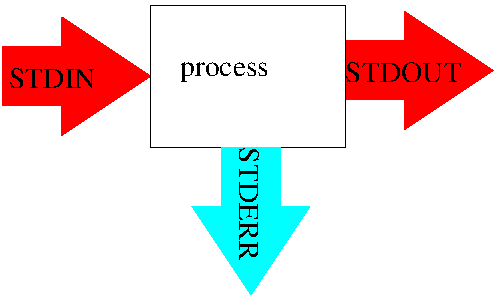
\includegraphics[width=1.2in]{process}
  \end{center}
  }
  \only<2>{
    \begin{center}
      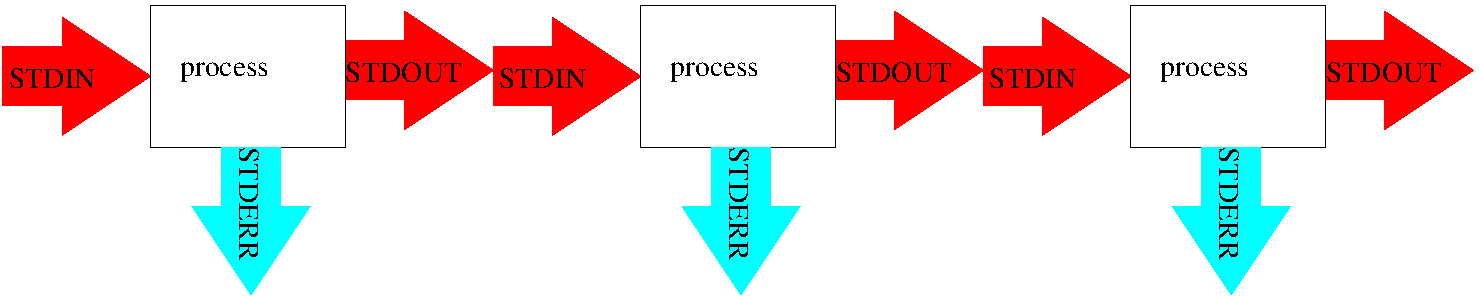
\includegraphics[width=3.6in]{processes}
    \end{center}
  }
  \begin{itemize}
    \item <1-> Каждое приложение открывает 3 стандартных файловых дескриптора stdin (fd 0), stdout(fd 1), stderr (fd 2)
    \item <2-> Приложения могут работать как фильтр из STDIN в STDOUT, можно объединять несколько приложений в конвейер
    \item <2-> Синтаксис {\tt <app1> | <app2>}
  \end{itemize}
\end{frame}

\begin{frame}{Дополнительный набор команд}
  \begin{itemize}
    \item {\tt cat} - Вывод файла в stdout, соединение нескольких файлов в stdout
    \item {\tt wc} - подсчет статистики символов в файле или в stdin 
    \item {\tt sort} - сортировка строк файла
    \item {\tt uniq} - объединение одинаковых строк в одну
    \item {\tt tr} - замена набора символов
    \item {\tt less} - программа-пейджер
    \item {\tt grep} - поиск строк, соответствующих регулярному выражению
    \item {\tt cut} - выделение полей из строк stdin
    \item {\tt awk} - небольшой язык программирования (также полезен для выделения полей)
  \end{itemize}
\end{frame}

\begin{frame}[fragile]{Некоторые примеры использования}
\begin{lstlisting}[language=bash]
cat /proc/1/environ | tr '\0' '\n' | less
ls  | wc -l # подсчет числа файлов
man uniq | tr  '[:space:]' '\n' | sort | uniq -c | sort -n | less # подсчет количества слов в тексте man uniq
history | wc -l # подсчет ранее введенных команд
cat /etc/udev/rules.d/* | wc -l
ls -s *.jpg | awk 'BEGIN{s=0};/^[ ]*[0-9]/{s+=\$1};END{print s}' 
\end{lstlisting}
  \pause
  \begin{block}{Упражнение}
    Посчитать статистику использования команд в history
  \end{block}
\end{frame}

\begin{frame}{Перенаправления в файл}

\begin{itemize}
  \item Перенаправление stdout 
    \begin{itemize}
      \item С созданием нового файла

        {\tt command > file} Например {\tt cat file1 file2 > file3}
      \item С дополнением существующего

		  {\tt command >\phantom{}>  file}
    \end{itemize}
    \pause
  \item Перенаправления stdin

    {\tt command < file}
    \pause
  \item Перенаправления stderr

    {\tt command1 2>\&1 | command2}

   {\tt command 1>file 2>\&1}

   {\tt command 2>file 1>\&2}
\end{itemize}

\end{frame}

\begin{frame}[fragile]{Мультистрочный ввод}

\begin{verbatim}
programm <<LABEL
Тут
    много
	     строк
LABEL
\end{verbatim}

	\pause
	\begin{block}{Пример}
	Передадим несколько строк в COM-порт 1
\begin{lstlisting}[language=bash]
cat >/dev/ttyS0 <<E_O_F
ATZ
ATDT 8w0170123456
E_O_F
\end{lstlisting}
	\end{block}
\end{frame}

\begin{frame}{Дополнительный набор команд для работы с текстом}
	\begin{itemize}
	  \item {\tt head} -- вывести первые строки
	  \item {\tt tail} -- вывести последние строки
		\begin{itemize}
			\item {\tt -f} -- отслеживать добавление данных в файл 
		\end{itemize}
	  \item {\tt tee} -- копировать стандартный вывод в файл
	  \item {\tt grep} -- печать текста, соответствующего шаблону
		\begin{itemize}
			\item {\tt -i}	
			\item {\tt -v}
			\item {\tt -o}
		\end{itemize}
	\end{itemize}
\end{frame}

\begin{frame}{Редакторы}
\begin{itemize}
 \item Интерактивные
 \begin{itemize}
 \item vi
   \begin{itemize}
    \item Есть почти везде
   \end{itemize}
 \item vim
 \item emacs
 \end{itemize}
 \item Поточные
	 \begin{itemize}
		 \item {\tt ed}
		 \item {\tt sed}
		 \item {\tt awk}
	\end{itemize}
 \end{itemize}
\end{frame}

\begin{frame}[fragile]{Метасимволы}
	\begin{block}{grep, sed, awk}
	\end{block}
	\begin{itemize}
		\item {\tt .} -- любой символ за исключением пустой строки
		\item {\tt *} -- любоe количество символов, которые стоят перед {\tt *}
		\item {\tt \^{}} -- начало строки
		\item {\tt \$} -- конец строки
		\item {\tt [...]} -- любой символ из заключенных в скобки
	\end{itemize}
\end{frame}

\begin{frame}[fragile]{sed}
	\begin{block}{Сценарии}
		{\tt [ addr [ ,  addr ] ] cmd [ args ]}
	\end{block}

	\small
	\begin{block}{Команды}
		\begin{itemize}
		  \item {\tt a, i} -- добавить строку после (перед) текущей
			  \begin{verbatim} who | sed -e 'a Text' \end{verbatim}
		  \item {\tt c} -- удалить строку и заменить на текст
			  \begin{verbatim} who | sed -e '/altlinux/ c Юзверь' \end{verbatim}
		  \item {\tt d} -- удалить строку
			  \begin{verbatim} who | sed -e '2,4 d' \end{verbatim}
			  \begin{verbatim} who | sed -e '/pts/ d' \end{verbatim}
		  \item {\tt s} -- замена по регулярному выражению
			  \begin{verbatim} who | sed -e 's/pts/консолька/g' \end{verbatim}
		\end{itemize}
	\end{block}
\end{frame}


\begin{frame}[fragile]{Практика: работа с текстовыми файлами}
  \begin{enumerate}
	  \item Посмотреть вывод команды {\tt dmesg}
	  \item Вывести на экран первые 10 строк 
		  \pause
	  \item Создать директорию в {\tt /tmp} и перейти в нее
	  \item Скопировать в файл1 последние 100 строк из {\tt /var/log/messages}
	  \item Запустить отслеживание изменений в файле1 на отдельной консоли
	  \item Дописать в файл1 из файла {\tt /etc/services}) все строки,
		  содержащие слова {\tt mail} или {\tt cache}
		  \pause
	  \item Запустить отслеживание изменений одновременно в файле1 и в {\tt /var/log/messages}\\
		  \pause
			повторить предыдущий пункт, убрав все комментарии при помощи {\tt sed}\\
		  \pause
		  ... и добиться параллельного вывода результатов на экран и во временный файл
	  \item
  \end{enumerate}
\end{frame}

\begin{frame}{Практика: работа с файловыми объектами}
	\begin{enumerate}
		\item Cкопировать файл1 в файл2
			\pause
		\item Добиться того, чтобы файл2 состоял из 3 одинаковых копий файла1
		\item Создать жесткую ссылку на файл1
		\item Создать символическую ссылку на файл2
		\item Вывести на экран список всех файлов
			\pause
		\item Добавить вывод команды {\tt date} в файл1
		\item Вывести на экран список всех файлов
		\item Вывести на экран содержимое файла1 и жесткой ссылки
		\item Создать именованный канал (PIPE)
		\item Запустить одну команду {\tt cat} на чтение из PIPE
		\item Записать содержимое файла1 и файла2 в PIPE
		\item Удалить временную директорию
	\end{enumerate}
\end{frame}

\begin{frame}{VI}
	\begin{block}<1>{Два режима работы}
		\begin{itemize}
			\item все портить
			\item бибикать
		\end{itemize}
	\end{block}
	\pause
	\begin{block}<2->{Два режима работы}
		\begin{itemize}
			\item командный 
			\item текстового ввода
		\end{itemize}
	\end{block}

	\begin{block}<2->{Переход между режимами}
		\begin{itemize}
			\item из командного в текстовый: i, a, R (вставка, добавление, замена)
			\item из текстового в командный: ESC или Ctrl-[
		\end{itemize}
	\end{block}

\end{frame}

\begin{frame}{VI: command mode}

	\begin{block}{Перемещение курсора}
		\begin{itemize}
			\item h, j, k, l -- влево, вниз, вверх, вправо (1 элемент)
			\item \^{} или 0 -- в начало строки
			\item \$ -- в конец строки
			\item w, b -- вперед, назад на слово
			\item gg, G -- начало, конец текста (<num>G -- на строку <num>)
		\end{itemize}
	\end{block}

	\begin{block}{Редактирование}
		\begin{itemize}
			\item d -- удалить (d -- текущую строку, w -- слово)
			\item u -- отмена предыдущего изменения
			\item . -- повтор
		\end{itemize}
	\end{block}
\end{frame}

\begin{frame}{VI: command mode}

	\begin{block}{Работа с неименованым буфером}
		\begin{itemize}
			\item y -- удалить (d -- текущую строку, w -- слово)
			\item p -- вставить из буфера
		\end{itemize}
	\end{block}

	\begin{block}{Командная строка}
		: -- переход в режим командной строки
		\begin{itemize}
			\item :q или :q! -- выход без сохранения
			\item :w -- сохранить изменения
			\item :x -- выйти с сохранением (:wq)
		\end{itemize}
	\end{block}
\end{frame}

\begin{frame}{Задание на дом}
\begin{block}{}
vimtutor ru
\end{block}
\end{frame}

%\begin{frame}{Настройки bash и кастомизация}
%  \begin{itemize}
%    \item Login shell
%      \begin{itemize}
%        \item {\tt /etc/profile}
%        \item {\tt $\sim$/.profile }
%      \end{itemize}
%    \item Обычная интерактивная shell
%      \begin{itemize}
%        \item {\tt /etc/bash.bashrc}
%        \item {\tt $\sim$/.bashrc}
%      \end{itemize}
%  \end{itemize}
%
%  Полезные команды
%  \begin{itemize}
%    \item {\tt alias}
%    \item {\tt export PATH=}
%    \item {\tt Определение функции}
%    \item {\tt shopts}
%  \end{itemize}
%
%\end{frame}

\begin{frame}{Архивация}
	\begin{block}{Архивация: tar}
		\begin{itemize}
			\item {\tt -c} -- создать архив
			\item {\tt -x} -- извлечь из архива
				\begin{itemize}
					\item {\tt -C} -- перейти в директорию
				\end{itemize}
			\item {\tt -f} -- запись в файл
		\end{itemize}
	\end{block}

	\begin{block}{Сжатие: gzip, bzip, xz}
		\begin{itemize}
			\item {\tt -[1-9]} -- изменить уровень сжатия
			\item {\tt -d} -- распаковать
			\item {\tt -c} -- вывод на консоль
		\end{itemize}
	\end{block}
\end{frame}

\begin{frame}[fragile]{Архивация: примеры}

	Создать сжатый архив:
	\begin{verbatim}
tar -czf archive.tar.gz *
	\end{verbatim}
	\pause
	Распаковать сжатый архив в директорию {\tt /tmp}:
	\begin{verbatim}
tar -C /tmp/ -xzf archive.tar.gz 
	\end{verbatim}
	\pause
	Создать сжатый архив:
	\begin{verbatim}
tar -czf archive.tar.gz *
	\end{verbatim}
	\pause
	Создать копию текущей директории в директории {\tt /tmp/copy/}:
	\begin{verbatim}
tar -c * | tar -C /tmp/copy -x
	\end{verbatim}
	\pause
	Создать копию текущей директории на другом хосте:
	\begin{verbatim}
HostDest: netcat -l 2222 | gzip -dc | tar -C /tmp/copy/ -x
HostSrc:  tar -c * | gzip -9 | netcat HostDest 2222
	\end{verbatim}
\end{frame}

\begin{frame}[fragile]{Поиск файлов}
	\begin{block}{find}
		\begin{itemize}
			\item {\tt -type} -- тип файлового объекта
			\item {\tt -size} -- размер
			\item {\tt -maxdepth} -- глубина рекурсии
			\item {\tt -exec} -- выполнить команду
			\item {\tt -printf} -- форматированный вывод
		\end{itemize}
	\end{block}

	\begin{block}{Примеры}
		\begin{verbatim}
find /etc -type f -size +100k  -exec ls -l {} \;
		\end{verbatim}

		\begin{verbatim}
find -type d -user altlinux
		\end{verbatim}
	
	\end{block}
\end{frame}

\begin{frame}[fragile]{xargs}
	\begin{block}{xargs}
			Утилита для создания и запуска команд из стандартного потока ввода:
		\begin{verbatim}
xargs [options] command [command options]
		\end{verbatim}
	
	\end{block}

	\begin{block}{Примеры}
		\begin{verbatim}
find /etc -type f -size -100k | xargs tar -czf /tmp/archive-100k.tar.gz
		\end{verbatim}

		\begin{verbatim}
find /etc -type f | xargs -I {} echo "Найден {} файл"
		\end{verbatim}
	
	\end{block}
\end{frame}


\end{document}
